\chapter{My Image Editor}

This application (cf. \ref{figure:ewc-image_editor} p.\pageref{figure:ewc-image_editor}) could be compared to a standard image editor like Photoshop or The Gimp. It offers lot of possibilities to edit images (rotation, styles, filters ...). This big advantage of My Image Editor is that it does not require any installation on your computer (only the Adobe flash player and a web browser are required). A second strenght is that it can be used standalone (\url{http://myimageeditor.moreedits.com/Editor/editor.php}) or integrated to the Easy Web Content platform.


\begin{figure}[!h]
\centering
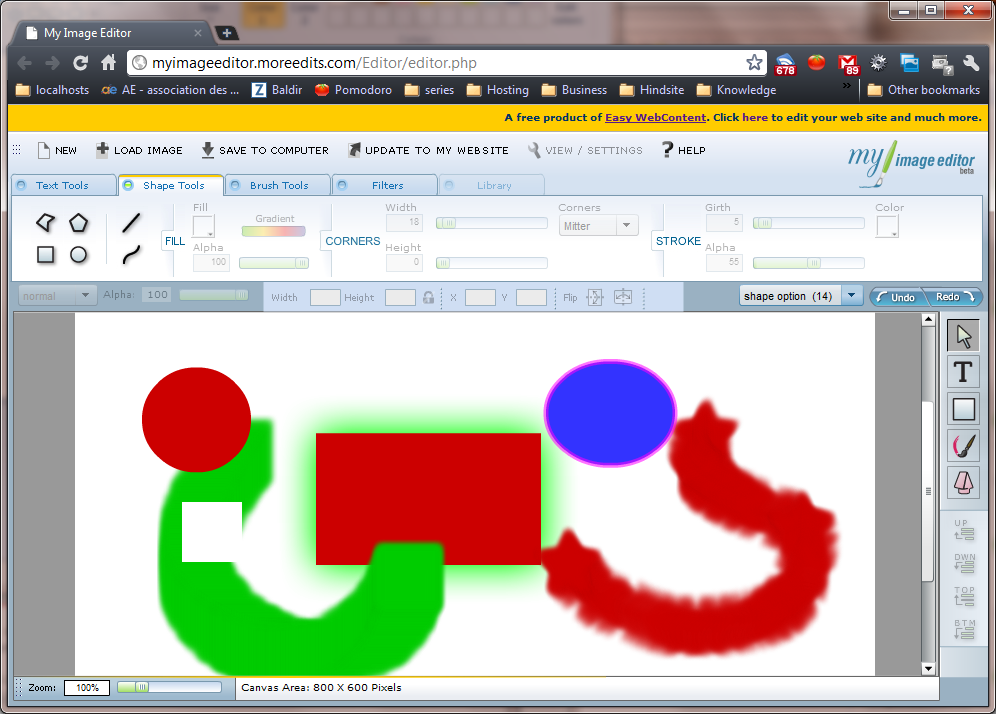
\includegraphics[width=.80\textwidth]{img/my_image_editor.png}
\caption{My Image Editor}
\label{figure:ewc-image_editor}
\end{figure}

I had first to "enter" head-first into the code written by the 3 previous interns. I was not very familiar with the Actionscript 3 programmation language but it is very similar to Java which I know better. One of the bigger difficulties was to deal with a main class file of more than 6000 lines of code. I could not refactor\footnote{Refactoring is a disciplined technique for restructuring an existing body of code, altering its internal structure without changing its external behavior (Martin Fowler \url{http://www.refactoring.com/)}} this piece of code because it would need too much time. 

I had to secure the swf file\footnote{file generated by Flash that can be embedded in a web page} by  using some URL rewrite technique and server side processing with PHP. Basically a PHP file with the .swf extension is used to import the file stream of the flash file. I added server directives to make .swf files interpreted as PHP scripts instead of directly downloaded. The PHP script require a session which is created by the script which want to embed the flash object. If the session is not found (which means that someone want to download the original .swf file by from its url it will return an error page instead of the file).

\lstset{language=PHP}
\begin{lstlisting}[label=swf-secure,caption=PHP script disguised into a swf file to avoid direct download]
	//retrieve the session
	session_start();
	//Test if the variable"flash" is directly access to prevent direct access by typing
	//the url of the swf file in the browser
	if(isset($_SESSION["flash"]))
	{
		$referrer = $_SERVER["HTTP_REFERER"];
		$referrer = parse_url($referrer);

		//Test if the domain are the same to prevent the access for others domains
		if($referrer["host"] != $_SESSION["flash"])
		{
			echo "Permission denied.";
			exit();
		}

	}
	else
	{
		echo "Permission denied.";
		exit();
	}
	//Destroy the session
	unset($_SESSION["flash"]);
	//Get the SWF if the test	
	header ("Cache-Control: no-cache, must-revalidate");
	header("Content-Type: application/x-shockwave-flash");
	readfile($_SERVER["DOCUMENT_ROOT"].'/Editor/01_Template.swf');
\end{lstlisting}
%$


I also had to add a preloader(cf. \ref{figure:ewc-image_preloader} p.\pageref{figure:ewc-image_preloader}) to the page embedding My Image Editor. The aim of this manipulation is to show a loading animation instead of a blank page while witing that the complete editor and its assets are fully loaded. In order to achieve this task the Image Editor had to communicate its status to the embedding page through a library called ExternalInterface. 

\begin{figure}[!h]
\centering
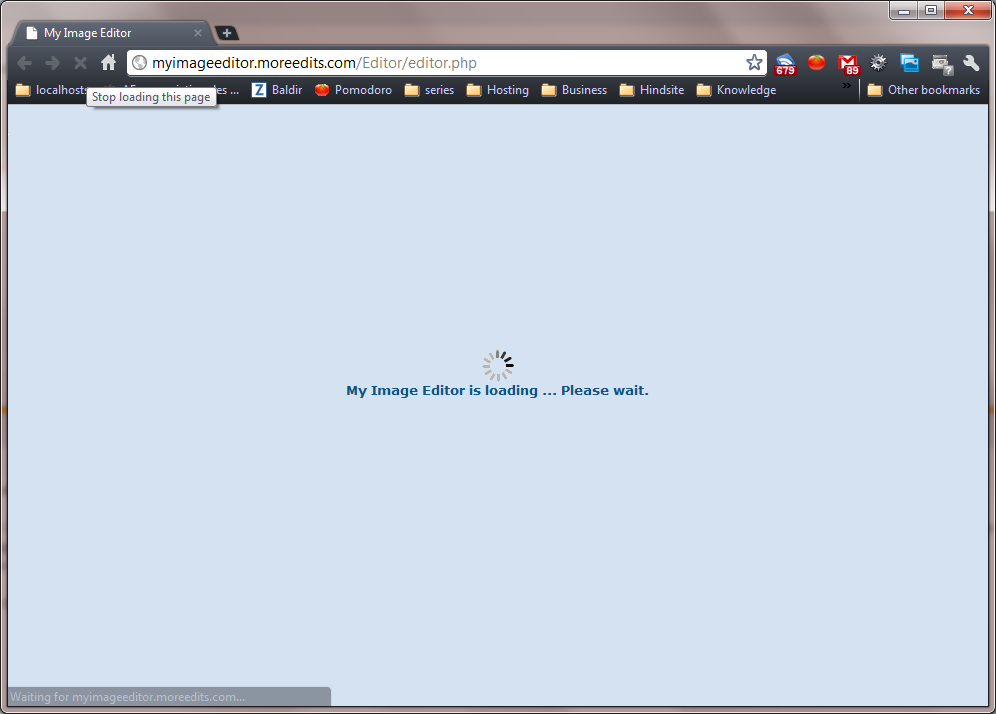
\includegraphics[width=.80\textwidth]{img/myimage_preloader.png}
\caption{My Image Editor preloader}
\label{figure:ewc-image_preloader}
\end{figure}

The other tasks were more flash related. Most of them were just little bug fixes such as brush issues, internal preloader, link to page, etc ...

After I worked enough on My Image Editor I continue to work on this project in parallel with the main project.